\documentclass[11pt,a4paper]{article}

\usepackage[utf8]{inputenc}
\usepackage[T1]{fontenc}
\usepackage{lmodern}
\usepackage[margin=2.5cm]{geometry}
\usepackage{amsmath,amssymb}
\usepackage{graphicx}
\usepackage{booktabs}
\usepackage{caption}
\usepackage{float}
\usepackage[authoryear,round]{natbib}
\usepackage[hidelinks]{hyperref}

\graphicspath{{figures/}}

\title{Predicting Consumer Loan Default with Machine Learning\\
\large From a Scorecard Benchmark to IFRS~9 Expected Credit Losses on 620{,}000 Lending Club Loans}
\author{Andreas Kyrlakis\\
\small MSc in Finance, HEC Lausanne (University of Lausanne)}
\date{November 2026}

\begin{document}
\maketitle

\begin{abstract}
\noindent
This paper builds a probability-of-default (PD) model for unsecured consumer loans and carries it through to the two decisions a lender takes with it: the expected credit loss (ECL) booked under IFRS~9 and the approval cut-off. The data are 620{,}779 real 36-month Lending Club loans issued between 2007 and 2015, all of which have either been repaid or charged off. The sample is split in time: training on loans issued up to 2014, validation on the first half of 2015 and test on the second half. A weight-of-evidence (WoE) logistic scorecard, the industry benchmark, reaches a test AUC of 0.650 (Gini 0.300). Six machine-learning models tuned by shuffled five-fold cross-validation do better: LightGBM reaches 0.673 (Gini 0.347, 95\% bootstrap interval 0.339--0.354), a gain of 0.023 AUC over the scorecard with a paired bootstrap interval of 0.021--0.025; a multilayer perceptron is statistically tied and wins on the validation set. After isotonic recalibration on the most recent period, the expected calibration error on the test set falls from 1.13 to 0.34 percentage points. SHAP values show that the FICO score, income, loan purpose and recent credit inquiries drive the predictions. The score is stable (PSI below 0.10 up to the end of 2018). Applied to the test portfolio at 30 June 2016, with an empirical LGD of 89\% from realised recoveries, an empirical default-timing curve and three unemployment scenarios, the probability-weighted ECL is USD 75.4 million, or 5.0\% of an exposure of USD 1.52 billion. A back-test against the losses that actually occurred afterwards shows that the model under-predicts the realised loss by 16\%. Finally, with costs measured on realised loan cash flows, the Bayes-optimal cut-off is a PD of 31.5\%; it refuses 2\% of applicants and raises the realised profit of the book by 0.9\%.
\end{abstract}

\section{Introduction}

A lender uses a probability of default for three things. It decides whether to grant the loan (the cut-off), it prices the loan, and, since 2018, it books a loss allowance for the loan from the day it is granted, as required by IFRS~9 \citep{ifrs9}. The allowance is the expected credit loss: over the next twelve months for performing loans, over the whole remaining life for loans whose credit risk has increased significantly \citep{bcbs2015}. The PD model therefore has to do more than rank borrowers: its probabilities must be calibrated, explainable to a validator, stable over time, and convertible into PDs over arbitrary horizons.

Machine learning has been compared with the logistic scorecard on many credit data sets; gradient boosting and ensembles usually win, but by margins that are small in absolute terms \citep{lessmann2015}. This paper asks the same question on a large public data set of real loans, with a time-based split that mimics how a model is used, and then goes further than most comparisons by following the PD into the ECL and into the approval decision. The questions are:
\begin{enumerate}
  \item How much better than a WoE scorecard do tree ensembles and a neural network rank borrowers, and is the difference statistically significant?
  \item Are the predicted PDs calibrated on a later period, and how should they be recalibrated?
  \item Which characteristics drive the predictions, for the portfolio and for one client?
  \item Is the score stable over time and across segments?
  \item What ECL does the model imply for a real portfolio under IFRS~9, and how does it compare with the losses that actually happened?
  \item Where should the approval cut-off be set when refusing a good client and accepting a bad one have different costs?
\end{enumerate}

\section{Data}

\subsection{Source}
Lending Club, a US peer-to-peer lender, published the full history of its loans. The file used here covers every loan issued from June 2007 to December 2018 (2.26 million loans, 151 columns, 1.7~GB) and is downloaded without an account from a public mirror under a CC0 licence (Hugging Face, \texttt{codesignal/lending-club-loan-accepted}). Larger and more representative data sets exist, notably the Freddie Mac single-family loan-level data and the Home Credit data on Kaggle, but both require an account and were not used.

\subsection{Sample and target}
I keep individual (not joint) loans with a 36-month term: 1{,}539{,}979 loans. A loan is in default if its final status is \emph{charged off} (or \emph{default}); it is good if it was \emph{fully paid}. The data end in December 2018, so every 36-month loan issued up to December 2015 has reached maturity: only 147 of the 620{,}926 loans issued in 2007--2015 are still unresolved, and they are dropped. Restricting the sample to fully observed vintages avoids the classic bias of Lending Club studies that keep recent vintages, where only the early defaults are visible. The modelling sample has 620{,}779 loans and a default rate of 13.9\%.

\subsection{Features}
Only information available at application is used (Table~\ref{tab:features}). Lending Club's own grade and interest rate are left out on purpose: they are the output of Lending Club's credit model, which used more bureau data than the public file contains. The sub-grade is kept as an external benchmark. The outcome columns (payments received, recoveries, last payment date) are never used as features; they serve only for the IFRS~9 part and for measuring profit.

\begin{table}[H]
\centering
\small
\caption{Application features (21). Missing values are imputed with the training median inside the model pipeline; ``months since last delinquency'' is set to 120 when the borrower was never delinquent.}
\label{tab:features}
\begin{tabular}{lp{11.5cm}}
\toprule
Group & Features \\
\midrule
Loan and income & loan amount, annual income, loan-to-income, debt-to-income (DTI) \\
Credit bureau & FICO (mid-point of range), credit history length, open accounts, total accounts, revolving balance and utilisation, inquiries in 6 months, delinquencies in 2 years, public records, bankruptcies, mortgage accounts, months since last delinquency \\
Applicant & employment length, home ownership, income verification, US region \\
Loan & purpose (debt consolidation, credit card, \ldots) \\
\bottomrule
\end{tabular}
\end{table}

\subsection{Split in time}
The loans are split on their issue date (Figure~\ref{fig:volume}): training 2007--2014 (337{,}992 loans, default rate 13.2\%), validation January--June 2015 (120{,}790 loans, 15.1\%) and test July--December 2015 (161{,}997 loans, 14.7\%). The test set is used once, at the end. The default rate rises over time as Lending Club opened its platform to riskier borrowers, which is exactly the situation in which a model trained on the past must be recalibrated.

\begin{figure}[H]
\centering
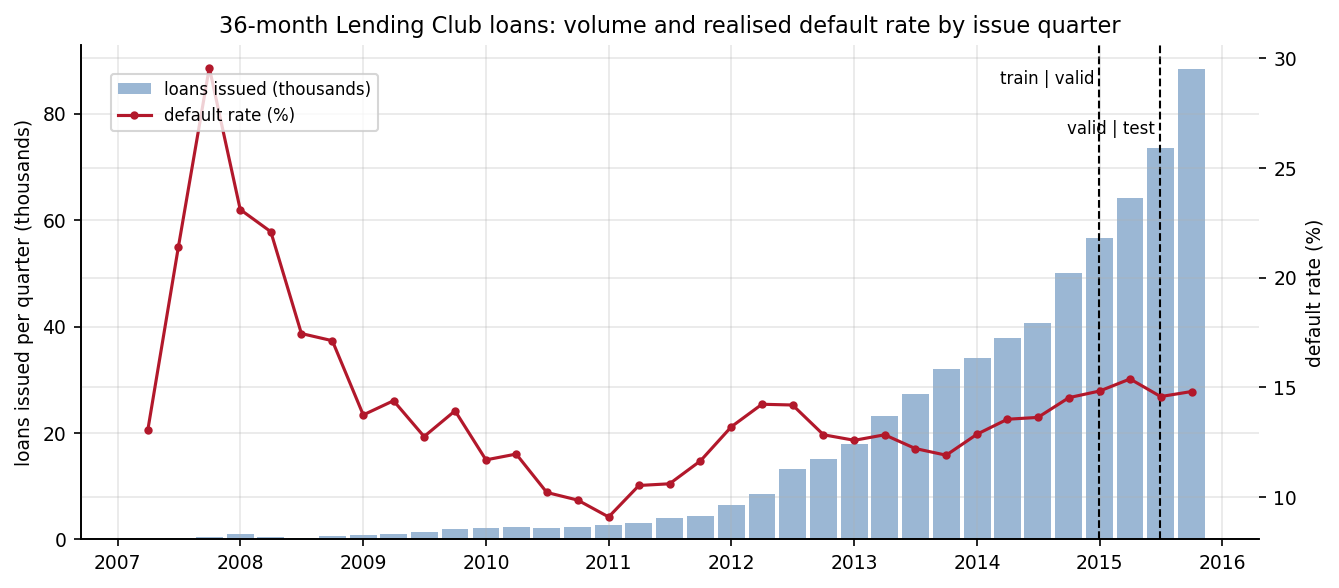
\includegraphics[width=0.9\textwidth]{fig01_volume_default_rate.png}
\caption{Volume and realised default rate by issue quarter, with the train/validation/test boundaries.}
\label{fig:volume}
\end{figure}

\section{Benchmark: the WoE scorecard}

\subsection{Method}
Each numeric feature is cut at its training deciles, and neighbouring bins are merged until the default rate is monotone in the feature; categories with less than 1\% of loans are pooled. For each bin, the weight of evidence and the information value \citep{siddiqi2017} are
\begin{equation}
\mathrm{WoE}_b = \ln\frac{g_b / G}{b_b / B}, \qquad
\mathrm{IV} = \sum_b \left(\frac{g_b}{G} - \frac{b_b}{B}\right)\mathrm{WoE}_b,
\end{equation}
where $g_b$ and $b_b$ are the numbers of good and bad loans in the bin (plus 0.5 to avoid empty cells) and $G$, $B$ the totals. A positive WoE marks a safer bin. Features with $\mathrm{IV} \ge 0.02$ enter a logistic regression on their WoE values, which is then turned into points: with a base of 600 points at good:bad odds of 50:1 and 20 points to double the odds,
\begin{equation}
\text{score} = 600 - \frac{20}{\ln 2}\ln 50 - \frac{20}{\ln 2}\Big(\beta_0 + \sum_j \beta_j \mathrm{WoE}_j\Big).
\end{equation}
The intercept is spread evenly across features so that each bin carries its own points.

\subsection{Results}
Nine features pass the IV filter (Figure~\ref{fig:iv}). The FICO score dominates (IV 0.139), followed by income (0.083), DTI (0.044) and loan-to-income (0.042); credit history length (0.019) and employment length (0.016) fall just below the threshold. All nine coefficients are negative, as they should be: a safer bin lowers the log-odds of default. On the test set the scorecard reaches an AUC of 0.650 and a Gini of 0.300 (Table~\ref{tab:models}); scores range from 511 to 587 points between the 1st and 99th percentiles. Lending Club's own sub-grade, mapped to its training default rate, reaches an AUC of 0.681 on the same loans: Lending Club saw more information than the public file contains.

\begin{figure}[H]
\centering
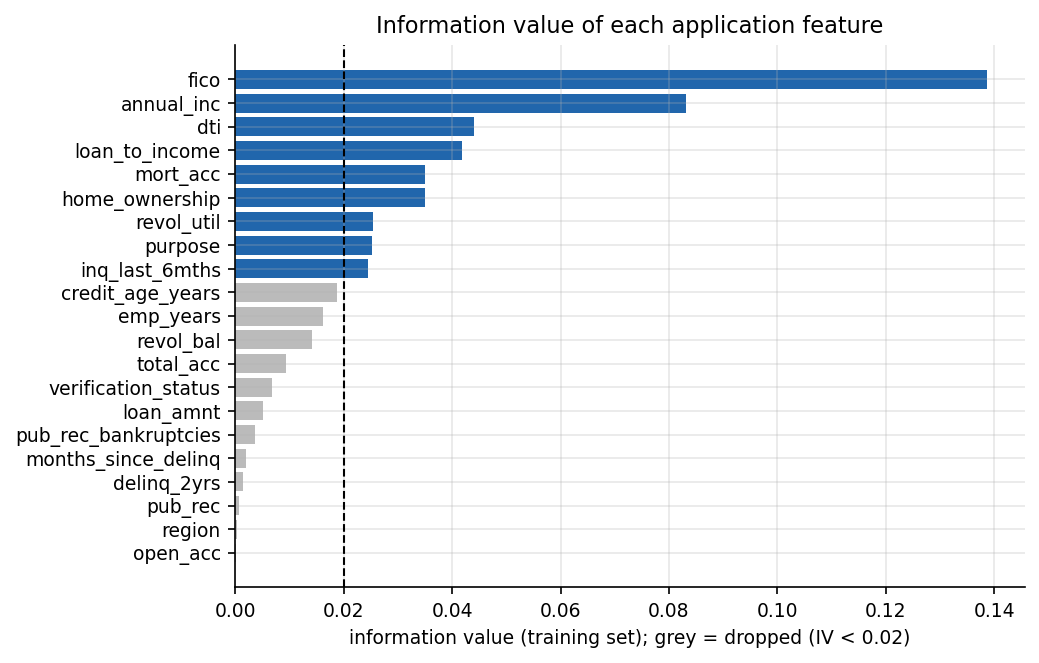
\includegraphics[width=0.62\textwidth]{fig03_information_value.png}
\caption{Information value of each feature on the training set; grey features are dropped.}
\label{fig:iv}
\end{figure}

\begin{figure}[H]
\centering
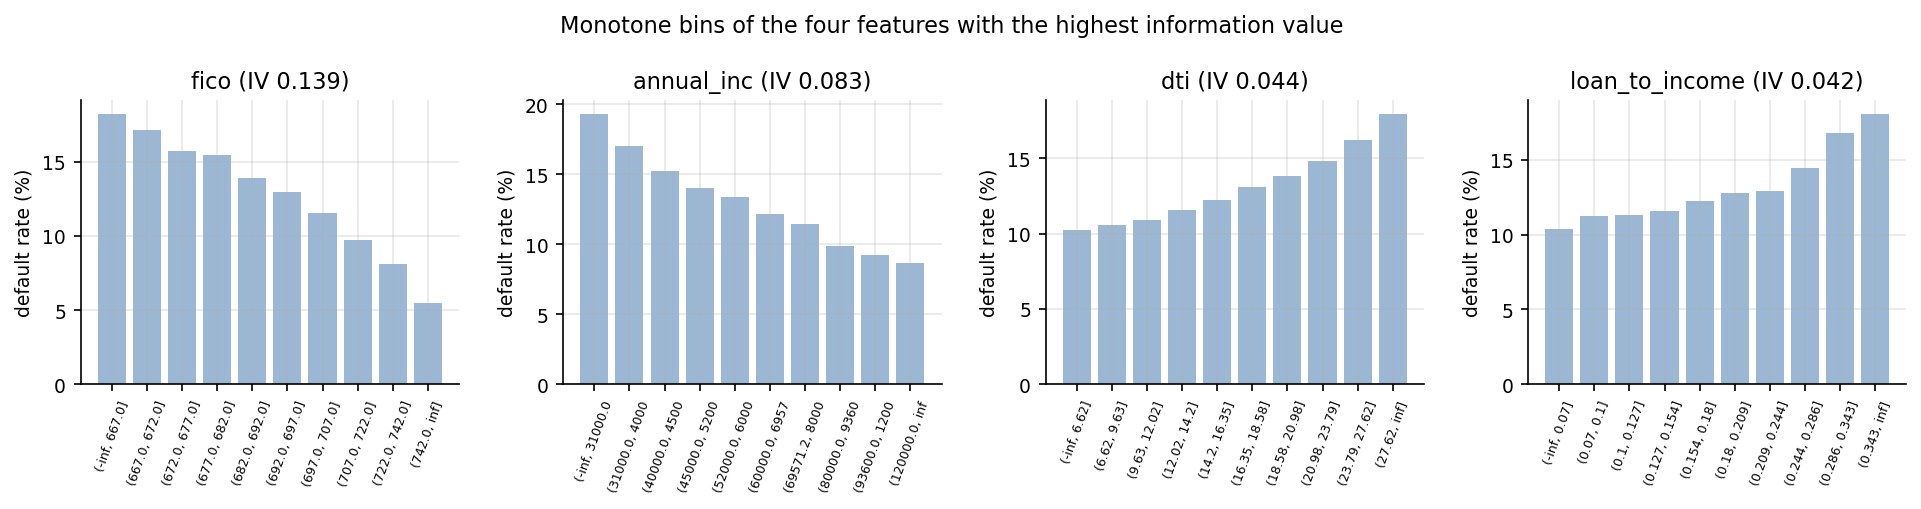
\includegraphics[width=\textwidth]{fig04_woe_bins.png}
\caption{Monotone bins and default rate of the four strongest features.}
\label{fig:woe}
\end{figure}

\section{Machine-learning models}

\subsection{Models and tuning}
Seven further models are compared with the scorecard: a logistic regression on the raw (log-scaled, standardised, one-hot) features; a decision tree; a random forest \citep{breiman2001}; scikit-learn's histogram gradient boosting; LightGBM \citep{ke2017}; a multilayer perceptron (MLP) with early stopping; and a soft vote averaging the PDs of the logistic regression, LightGBM and the MLP. All preprocessing (imputation, scaling, encoding) sits inside a scikit-learn pipeline \citep{pedregosa2011}, so it is learned on the training folds only.

Hyperparameters are chosen by randomised search (8 to 20 candidates per model) with five-fold, shuffled, stratified cross-validation on a random sample of 60{,}000 training loans, scored by AUC; the sample size is a CPU and memory budget. Each model is then refitted on all 337{,}992 training loans. The cross-validated AUCs range from 0.626 (tree) to 0.662 (LightGBM, 10 leaves, learning rate 0.024, 704 trees, row and column subsampling); the MLP selects two hidden layers of 128 and 64 units.

\subsection{Metrics}
For each model the test set gives the AUC, the Gini ($2\,\mathrm{AUC}-1$, the usual bank measure), the Kolmogorov--Smirnov statistic (largest gap between the score distributions of bad and good loans), the Brier score (mean squared error of the PD) and the area under the precision--recall curve, which is informative when defaults are the minority class. Each comes with a 95\% percentile interval from 300 bootstrap resamples of the test loans \citep{efron1979}. The difference between two models is tested with a paired bootstrap on the same resamples.

\begin{table}[H]
\centering
\small
\caption{Test set (161{,}997 loans issued July--December 2015). Values with 95\% bootstrap intervals for AUC and Gini. Lower Brier is better.}
\label{tab:models}
\resizebox{\textwidth}{!}{%
\begin{tabular}{lcccccc}
\toprule
Model & AUC & Gini & KS & Brier & PR-AUC & Valid. AUC \\
\midrule
LightGBM & 0.673 {\scriptsize[0.669, 0.677]} & 0.347 {\scriptsize[0.339, 0.354]} & 0.250 & 0.1198 & 0.250 & 0.668 \\
Soft vote (LR+LGBM+MLP) & 0.672 {\scriptsize[0.668, 0.676]} & 0.345 {\scriptsize[0.337, 0.352]} & 0.249 & 0.1198 & 0.250 & 0.667 \\
MLP & 0.672 {\scriptsize[0.668, 0.676]} & 0.344 {\scriptsize[0.336, 0.351]} & 0.249 & 0.1196 & 0.250 & 0.668 \\
Hist.\ gradient boosting & 0.669 {\scriptsize[0.665, 0.672]} & 0.338 {\scriptsize[0.331, 0.345]} & 0.243 & 0.1202 & 0.247 & 0.664 \\
Random forest & 0.668 {\scriptsize[0.664, 0.671]} & 0.336 {\scriptsize[0.328, 0.342]} & 0.244 & 0.1204 & 0.244 & 0.664 \\
Logistic (raw features) & 0.661 {\scriptsize[0.657, 0.665]} & 0.322 {\scriptsize[0.314, 0.330]} & 0.231 & 0.1206 & 0.239 & 0.656 \\
WoE scorecard & 0.650 {\scriptsize[0.646, 0.654]} & 0.300 {\scriptsize[0.293, 0.307]} & 0.217 & 0.1213 & 0.232 & 0.646 \\
Decision tree & 0.641 {\scriptsize[0.637, 0.644]} & 0.281 {\scriptsize[0.274, 0.288]} & 0.201 & 0.1219 & 0.219 & 0.635 \\
\midrule
LC sub-grade (benchmark) & 0.681 & 0.363 & 0.267 & 0.1198 & 0.251 & -- \\
\bottomrule
\end{tabular}}
\end{table}

\subsection{Results}
Table~\ref{tab:models} and Figure~\ref{fig:auc} give the ranking. The three best models --- LightGBM, the MLP and the vote --- are statistically indistinguishable: their intervals overlap almost entirely, and the vote is in fact 0.0009 AUC below LightGBM (paired interval $-0.0016$ to $-0.0001$). LightGBM beats the scorecard by 0.023 AUC (paired interval 0.021 to 0.025), i.e.\ 4.6 Gini points: a clear and significant gain, but a modest one in absolute terms, in line with the literature \citep{lessmann2015}. Half of the gain comes from using raw features instead of coarse bins (the raw logistic regression is 0.011 above the scorecard), the other half from non-linearities and interactions. The champion used in the rest of the paper is chosen on the validation set, not the test set: it is the MLP (validation AUC 0.6681 against 0.6676 for LightGBM).

\begin{figure}[H]
\centering
\begin{minipage}{0.56\textwidth}
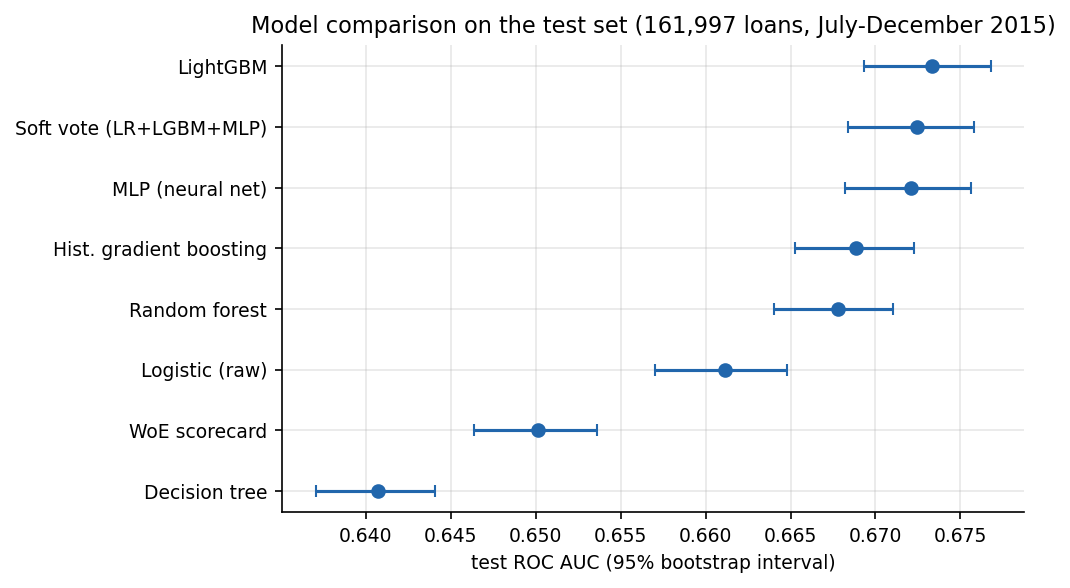
\includegraphics[width=\textwidth]{fig05_model_auc.png}
\end{minipage}\hfill
\begin{minipage}{0.42\textwidth}
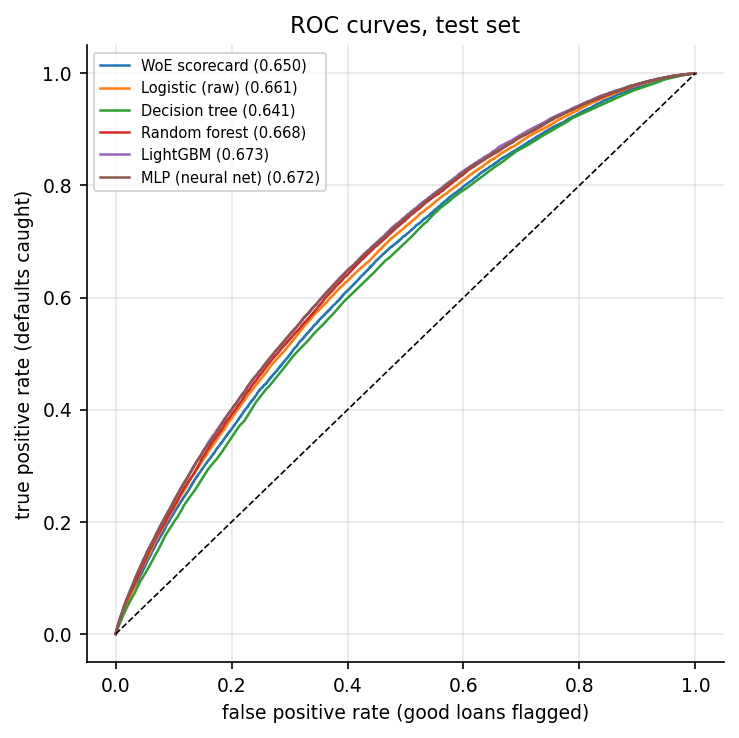
\includegraphics[width=\textwidth]{fig06_roc.png}
\end{minipage}
\caption{Left: test AUC with 95\% bootstrap intervals. Right: ROC curves.}
\label{fig:auc}
\end{figure}

\subsection{Learning curves}
Figure~\ref{fig:lc} refits the tuned logistic regression and LightGBM on random subsets of 2{,}000 to 337{,}992 training loans. The logistic regression is saturated after about 50{,}000 loans (validation AUC 0.656). LightGBM keeps improving up to 200{,}000 loans and its gap between training and validation AUC shrinks from 0.20 to 0.013, so it is not over-fitting at full size; the remaining gain from more data of the same kind would be small. The limit is the information in the features, not the sample size.

\begin{figure}[H]
\centering
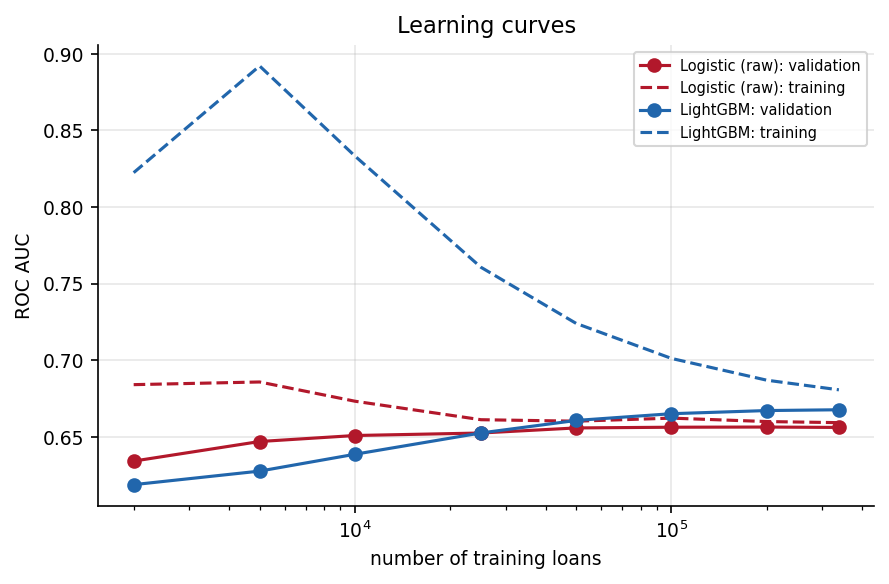
\includegraphics[width=0.6\textwidth]{fig07_learning_curves.png}
\caption{Learning curves: training (dashed) and validation (solid) AUC.}
\label{fig:lc}
\end{figure}

\section{Calibration}

A PD used for provisions and pricing must be a probability, not only a ranking. The MLP trained on 2007--2014 predicts an average PD of 13.6\% on the test set, while 14.7\% of the test loans default: the population drifted towards riskier borrowers. Two recalibrations are fitted on the validation period \citep{niculescu2005}: Platt scaling, a logistic regression of the outcome on the logit of the PD \citep{platt1999}, and isotonic regression, a monotone step function \citep{zadrozny2002}. The method is chosen on the validation set by five-fold cross-fitting (each fold calibrated on the other four): isotonic regression gives an expected calibration error (ECE, mean absolute gap between predicted and observed default rate over ten deciles) of 0.550 percentage points against 0.569 for Platt, so isotonic is kept.

On the test set (Figure~\ref{fig:calib}), the raw PDs are too low in every decile (ECE 1.13 pp). Both recalibrations put the deciles on the diagonal: ECE 0.18 pp for Platt and 0.34 pp for isotonic, with the mean PD at 14.67\%. Platt would have been slightly better on the test set; the two were nearly tied on validation and the choice was not revisited after seeing the test. Platt's slope of 0.91 indicates slightly over-confident raw scores. Recalibration leaves the ranking unchanged (AUC 0.672) and improves the Brier score marginally.

\begin{figure}[H]
\centering
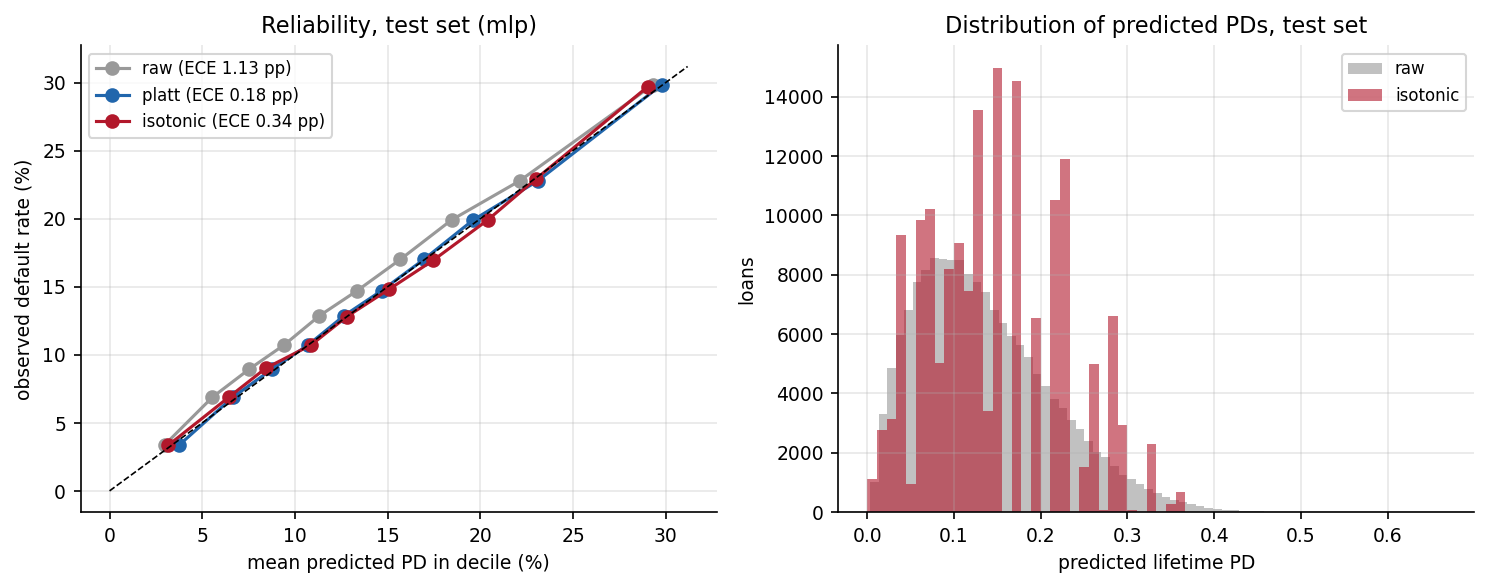
\includegraphics[width=\textwidth]{fig08_calibration.png}
\caption{Reliability diagram on the test set (deciles of predicted PD) and distribution of PDs before and after isotonic recalibration.}
\label{fig:calib}
\end{figure}

\section{Explaining the predictions}

SHAP values \citep{lundberg2017} split each prediction into additive contributions of the features. For tree ensembles they can be computed exactly and quickly \citep{lundberg2020}, so the explanation is computed for LightGBM, whose test AUC is within 0.0012 of the MLP champion, on 5{,}000 test loans. Contributions are in log-odds; for every loan, their sum plus the average log-odds reproduces the model output (maximum error $1.3 \times 10^{-14}$).

Globally (Figure~\ref{fig:shap}), the FICO score is the strongest driver (mean $|\mathrm{SHAP}|$ 0.30), followed by income (0.14), loan purpose (0.14), credit inquiries in the last six months (0.13), DTI (0.12) and loan-to-income (0.11). The directions are those a credit officer expects: a low FICO, many recent inquiries, a high DTI and a loan large relative to income raise the PD. Bankruptcies, public records and past delinquencies matter little once FICO is known, because FICO already contains them.

Locally (Figure~\ref{fig:waterfall}), the riskiest client in the sample who did default has a PD of 40.5\% against an average of 11.7\%. Four inquiries in six months add 0.42 to the log-odds, a loan of 39\% of a USD 30{,}600 income adds 0.32, a FICO of 672 adds 0.31 and a DTI of 30 adds 0.16. This is the reason-code output that consumer-credit rules require when an application is declined.

\begin{figure}[H]
\centering
\begin{minipage}{0.44\textwidth}
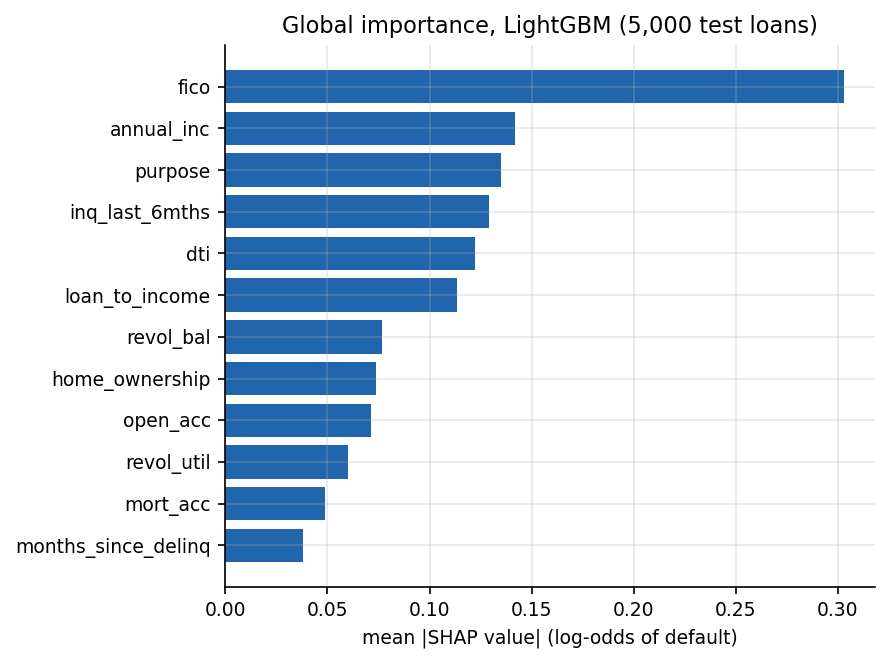
\includegraphics[width=\textwidth]{fig09_shap_importance.png}
\end{minipage}\hfill
\begin{minipage}{0.54\textwidth}
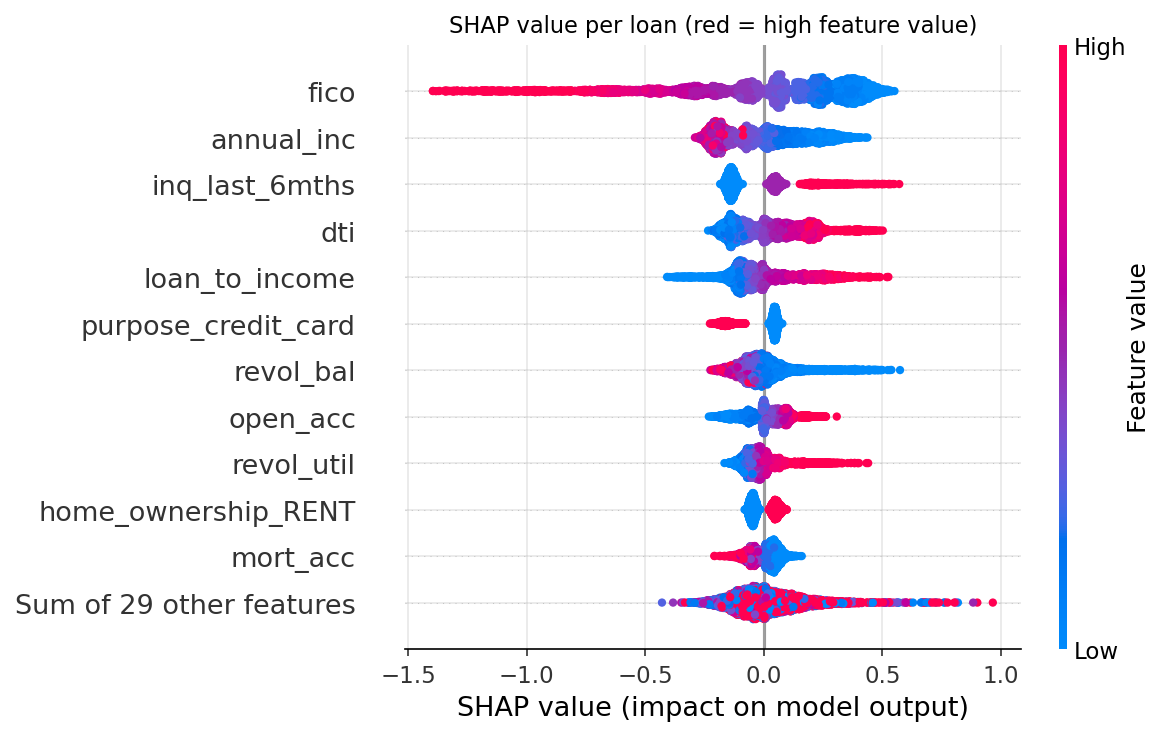
\includegraphics[width=\textwidth]{fig10_shap_beeswarm.png}
\end{minipage}
\caption{Global SHAP importance (one-hot columns grouped back to their feature) and SHAP value of each loan.}
\label{fig:shap}
\end{figure}

\begin{figure}[H]
\centering
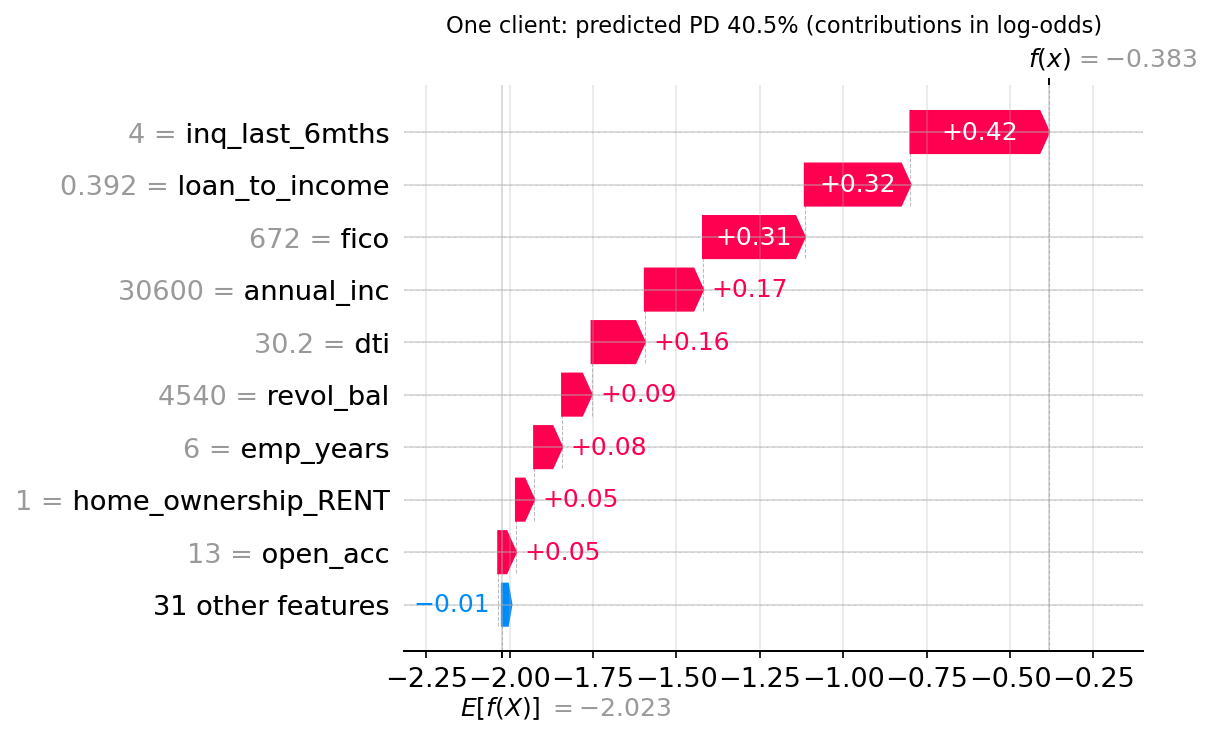
\includegraphics[width=0.7\textwidth]{fig11_shap_waterfall.png}
\caption{Local explanation for one client: from the average log-odds ($-2.02$) to the client's log-odds ($-0.38$, PD 40.5\%).}
\label{fig:waterfall}
\end{figure}

\section{Stability and performance by segment}

\subsection{Population stability}
The population stability index compares the distribution of the score in a new population with the training one, over the training deciles:
\begin{equation}
\mathrm{PSI} = \sum_{k=1}^{10} (a_k - e_k)\ln\frac{a_k}{e_k},
\end{equation}
read as stable below 0.10, to be monitored between 0.10 and 0.25 and shifted above 0.25 \citep{yurdakul2018}. The PSI needs no outcome, so the champion can be monitored on every quarter of applications up to the end of the data, including 2016--2018 loans whose outcome is not known yet (Figure~\ref{fig:psi}). The PSI is 0.004 for the validation set and 0.001 for the test set, and it rises slowly to 0.071 in 2018Q4 while the mean raw PD falls from 13.5\% to 11.6\%: Lending Club tightened its lending after 2016. The drift stays below the monitoring threshold. At the feature level, income verification moves the most between training and test (PSI 0.109): Lending Club verified more incomes over time.

\begin{figure}[H]
\centering
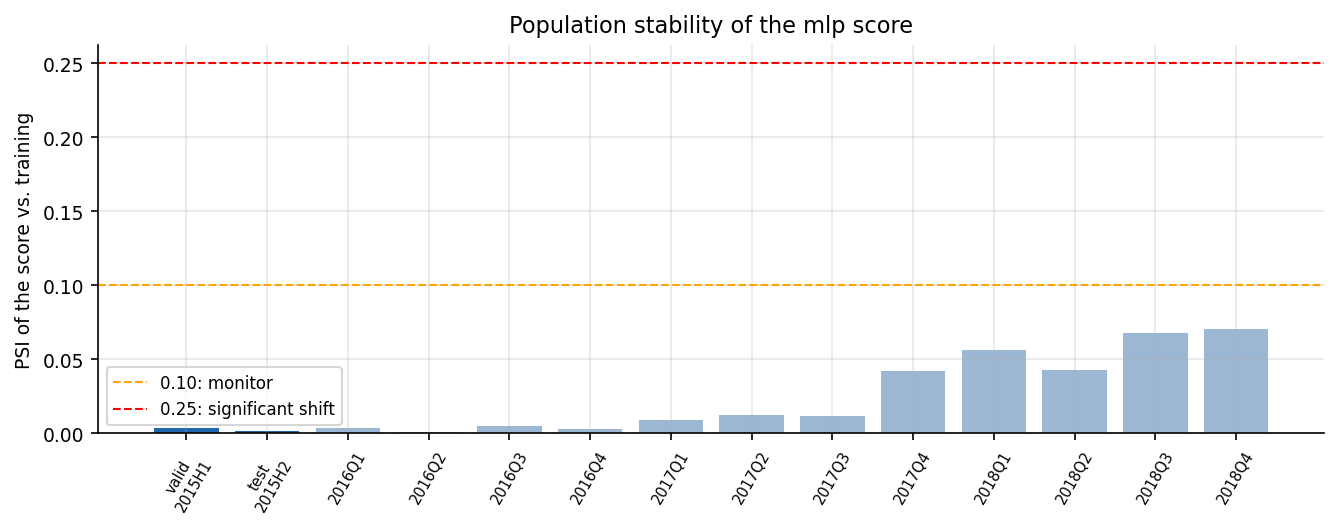
\includegraphics[width=0.9\textwidth]{fig12_psi.png}
\caption{PSI of the champion score against the training distribution, by period.}
\label{fig:psi}
\end{figure}

\subsection{Segments}
Lending Club holds no protected attribute (age, sex, ethnicity), so a full fair-lending analysis is not possible. Instead, Figure~\ref{fig:groups} checks discrimination and calibration by segment on the test set. The calibrated PD matches the observed default rate within one percentage point for every home-ownership type, region and income quintile. Discrimination is weaker for the lowest income quintile (AUC 0.633) than for the highest (0.690), and for renters (0.654) than for home-owners with a mortgage (0.677): the model separates risk less well where the population is more homogeneous on the strongest features. The one clear calibration gap is for applicants who did not state an employment length: 21.5\% default against 17.3\% predicted. Such a segment would be flagged for an overlay or a dedicated variable.

\begin{figure}[H]
\centering
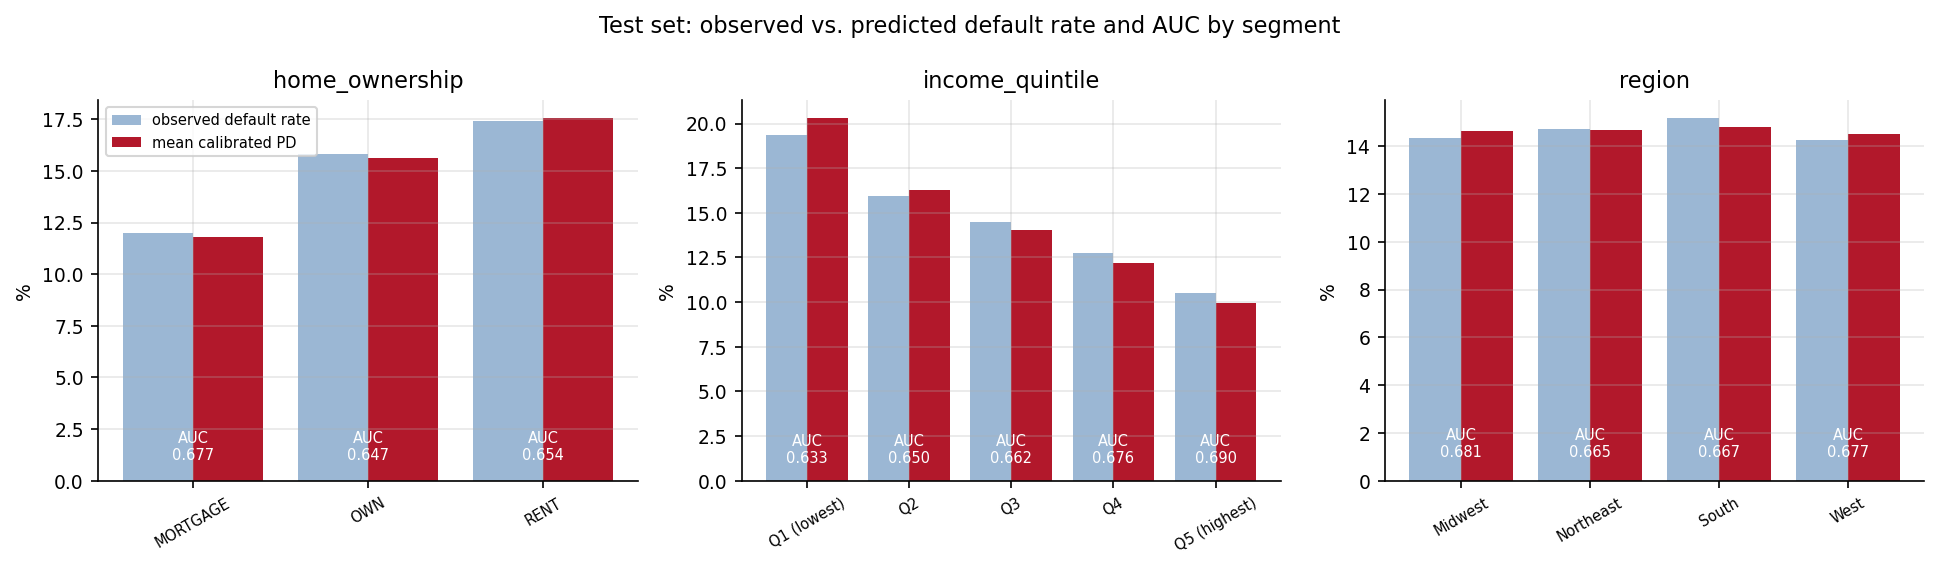
\includegraphics[width=\textwidth]{fig13_subgroups.png}
\caption{Observed default rate, mean calibrated PD and AUC by segment (test set).}
\label{fig:groups}
\end{figure}

\section{From PD to IFRS 9 expected credit losses}

\subsection{Portfolio and reporting date}
The test loans form the portfolio, seen at a reporting date of 30 June 2016, when they are 6 to 11 months old. Their status at that date is reconstructed from the data: 12{,}744 loans were already repaid early, 962 charged off, and 148{,}291 loans with an exposure of USD 1.52 billion are on the book. For the loans that eventually defaulted, the first missed payment is one month after the last payment received; this gives their days past due at the reporting date.

\subsection{Building blocks}
\paragraph{PD term structure.} The model gives a lifetime (36-month) PD $p$ at origination. Among the 44{,}472 training defaults, the share $F(m)$ that occurred by loan month $m$ gives the timing (Figure~\ref{fig:timing}): 31\% of defaults happen in the first year and 73\% in the first two. Assuming every loan shares this shape, the cumulative PD by month $m$ is $p\,F(m)$, and the PD over months $(a, a+h]$ for a loan still performing at age $a$ is
\begin{equation}
\mathrm{PD}(a, a+h) = \frac{p\,[F(a+h) - F(a)]}{1 - p\,F(a)}.
\end{equation}
At the reporting date the average 12-month PD is 6.6\% and the average remaining lifetime PD is 12.5\%.

\paragraph{EAD.} The exposure at default is the scheduled balance of the annuity loan just before the missed payment, from its amount, rate and term. Prepayments are ignored, which overstates the exposure of loans that will be repaid early.

\paragraph{LGD.} For each charged-off training loan,
\begin{equation*}
\mathrm{LGD} = 1 - \frac{\text{recoveries} - \text{collection fees}}{\text{principal outstanding at default}}.
\end{equation*}
 The exposure-weighted average is 89.2\% (median 90.2\%, Figure~\ref{fig:timing}): unsecured consumer loans recover little. Recoveries are not discounted because their timing is not in the data.

\paragraph{ECL.} For each loan, with monthly marginal PDs $q_k$, the loan's monthly rate $r$ as effective interest rate and scheduled balances $\mathrm{EAD}_k$,
\begin{equation}
\mathrm{ECL} = \sum_{k=1}^{H} q_k \cdot \mathrm{LGD} \cdot \mathrm{EAD}_k \cdot (1+r)^{-k},
\end{equation}
with $H = 12$ months in stage 1 and the remaining life in stage 2. In stage 3 (credit-impaired) the PD is one and $\mathrm{ECL} = \mathrm{LGD} \times \mathrm{EAD}$.

\paragraph{Staging.} A loan is in stage 3 if it is more than 90 days past due, in stage 2 if it is more than 30 days past due (the IFRS~9 backstop) or if its annualised remaining-life PD, weighted over the scenarios, is at least twice its annualised lifetime PD at origination; otherwise it is in stage 1. Without a monthly re-scoring of the borrowers, the relative test can only react to the scenarios and to the shape of the timing curve; it moves no loan here, so all 1{,}375 stage-2 loans come from the 30-day backstop.

\begin{figure}[H]
\centering
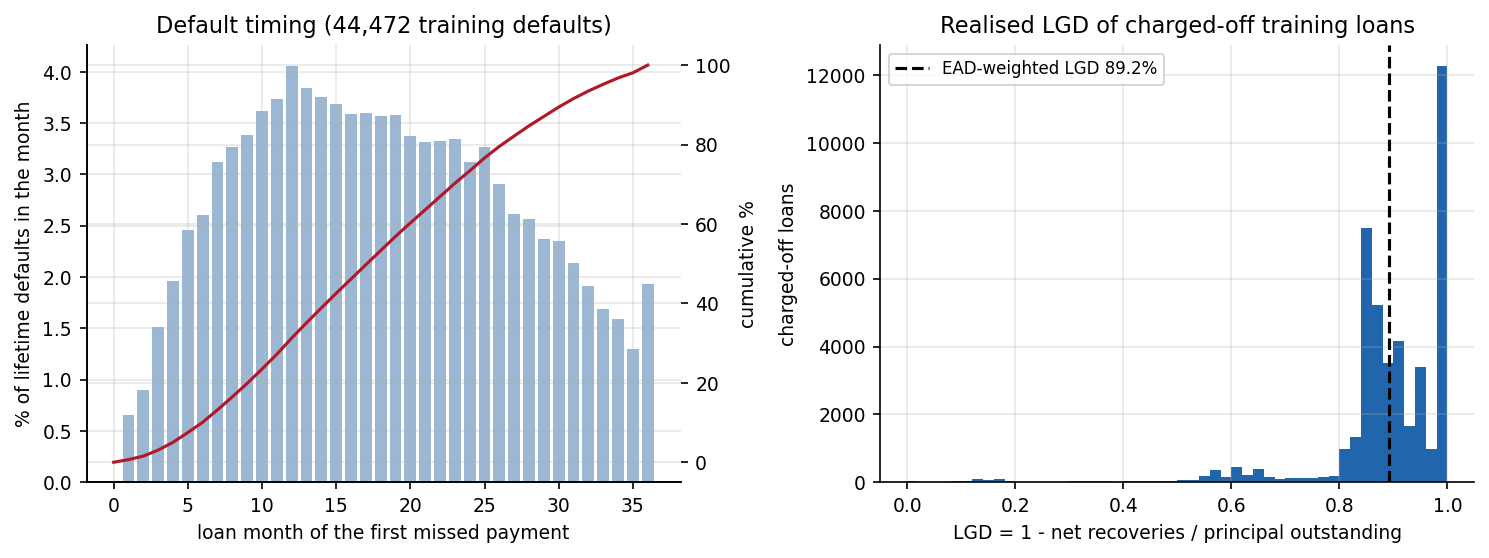
\includegraphics[width=\textwidth]{fig14_timing_lgd.png}
\caption{Left: month of the first missed payment of training defaults. Right: realised LGD of charged-off training loans.}
\label{fig:timing}
\end{figure}

\subsection{Forward-looking scenarios}
IFRS~9 requires the ECL to weigh several forward-looking scenarios. Lending Club's history is too short to estimate a macro link, so it is estimated on a longer series: the quarterly charge-off rate on consumer loans of US banks against the US unemployment rate (FRED, 1985--2026, 166 quarters, Figure~\ref{fig:macro}). A logit regression gives a slope of 0.065 per percentage point of unemployment. The fit is weak ($R^2 = 0.08$): over four decades the level of charge-offs also moved for reasons unrelated to unemployment, so the slope is a conservative, rough sensitivity. Each lifetime PD is shifted in logit space, $\mathrm{logit}\,p_s = \mathrm{logit}\,p + 0.065\,\Delta U_s$, under three scenarios whose weights and shocks are assumptions: upside ($-1$ pp, weight 15\%), base (unemployment stays at 4.9\%, 60\%) and downside ($+3$ pp, 25\%).

\begin{figure}[H]
\centering
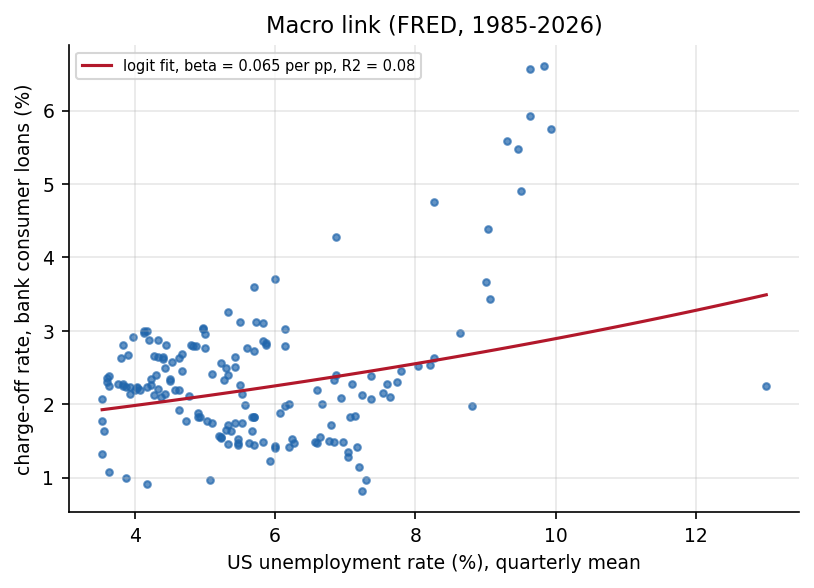
\includegraphics[width=0.5\textwidth]{fig15_macro_link.png}
\caption{Charge-off rate of US banks on consumer loans against unemployment, with the logit fit.}
\label{fig:macro}
\end{figure}

\subsection{Results}
Table~\ref{tab:ecl} and Figure~\ref{fig:ecl} give the result. The probability-weighted ECL is USD 75.4 million, a coverage of 5.0\% of the exposure. Stage~1 holds 98.4\% of the loans with a coverage of 4.4\%; stage~2 holds 1{,}375 loans at 8.1\%; the 937 stage-3 loans carry the full LGD of 89.2\%. Across scenarios the ECL ranges from USD 69.6 million (upside) to 84.5 million (downside); the weighted ECL is 3.2\% above the base scenario, the non-linearity that IFRS~9 asks banks to capture. Staging matters more than the scenarios: if every loan were provisioned over its lifetime the base ECL would be USD 88.9 million, against 65.4 million with 12-month ECL for all.

\begin{table}[H]
\centering
\small
\caption{ECL at 30 June 2016 on the test portfolio (probability-weighted).}
\label{tab:ecl}
\begin{tabular}{lrrrr}
\toprule
 & Loans & EAD (USD m) & ECL (USD m) & Coverage \\
\midrule
Stage 1 (12-month ECL) & 145{,}979 & 1{,}493.4 & 66.4 & 4.4\% \\
Stage 2 (lifetime ECL) & 1{,}375 & 13.7 & 1.1 & 8.1\% \\
Stage 3 (credit-impaired) & 937 & 8.9 & 7.9 & 89.2\% \\
\midrule
Total & 148{,}291 & 1{,}516.0 & 75.4 & 5.0\% \\
\midrule
Scenario ECL: upside / base / downside & \multicolumn{4}{r}{69.6 / 73.1 / 84.5} \\
\bottomrule
\end{tabular}
\end{table}

\begin{figure}[H]
\centering
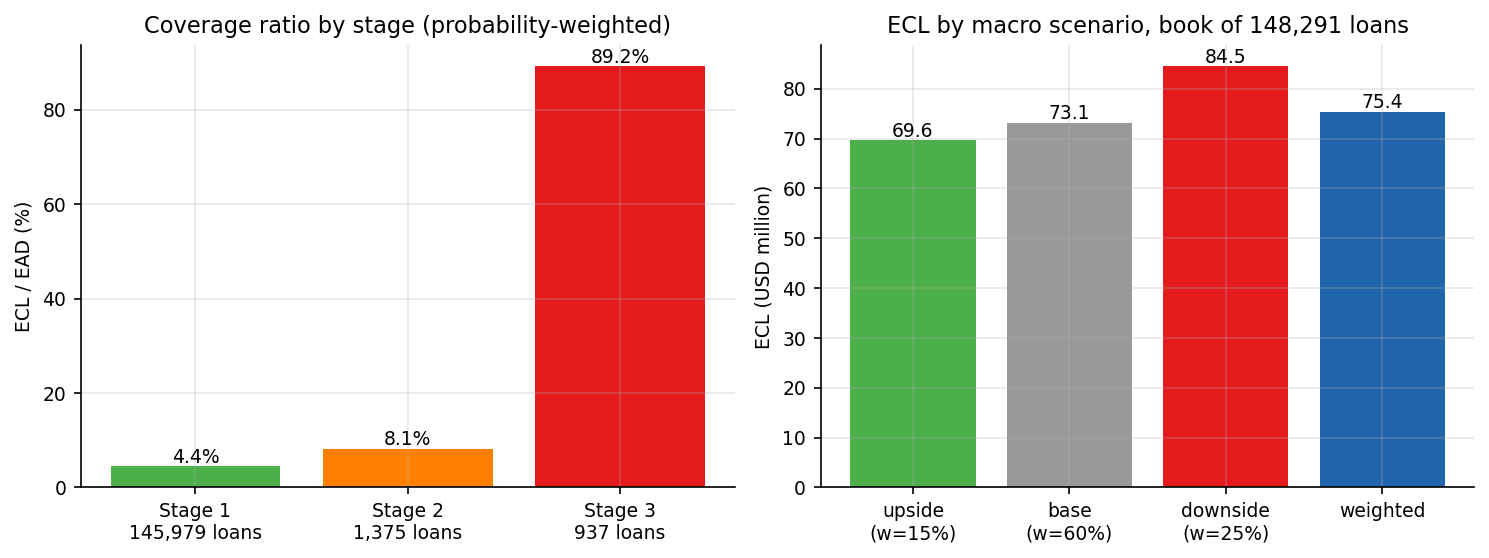
\includegraphics[width=\textwidth]{fig16_ecl.png}
\caption{Coverage by stage and ECL by scenario.}
\label{fig:ecl}
\end{figure}

\subsection{Back-test}
The data reveal what happened next. Of the 147{,}354 performing loans at the reporting date, 13.4\% defaulted before maturity, against a predicted remaining lifetime PD of 12.4\%. Their realised principal loss, net of recoveries, was USD 115.4 million; the undiscounted lifetime expected loss of the base scenario was USD 96.6 million, 16\% lower. About half of the gap comes from the PD (7\% too low in relative terms) and half from the loss per default (realised USD 5{,}860 against 5{,}270 expected). Two simplifications point in this direction: the delinquent stage-2 loans keep their origination PD instead of a much higher roll-rate PD, and the timing curve estimated on 2007--2014 vintages may not hold for the riskier 2015 vintages. A bank would correct both before using such a model, and this kind of back-test is how the gap is found.

\section{Choosing the approval cut-off}

Refusing a good applicant forgoes the margin on the loan; approving a bad one loses part of the principal. Both costs are measured on the realised cash flows of the training loans, as a share of the amount lent: a fully repaid loan earned on average 16.5\% (interest received over its life), and a charged-off loan lost 35.9\% (principal not repaid, net of interest received and recoveries). With calibrated PDs, the expected cost $c_{FP}\,(1-p) \mathbf{1}_{\text{refuse}} + c_{FN}\, p\, \mathbf{1}_{\text{accept}}$ is minimised by refusing when \citep{elkan2001}
\begin{equation}
p \ge p^* = \frac{c_{FP}}{c_{FP} + c_{FN}} = \frac{0.165}{0.165 + 0.359} = 31.5\%.
\end{equation}
The cut-off that minimises the empirical cost on the validation set is 31\%, which confirms the formula; the one that maximises realised profit on the validation set is 35.5\%.

Applied unchanged to the test set (Figure~\ref{fig:threshold}), the Bayes cut-off approves 98.0\% of applicants. The 2\% it refuses default at 37.5\%, against 14.2\% for the approved loans; the realised profit of the book rises from USD 131.8 million to 133.0 million (+0.9\%), and the profit per dollar lent from 6.35 to 6.52 cents. The gain is small for a simple reason: every loan in the data had already been approved and priced by Lending Club's own model, so the riskiest applicants never appear, and the high-PD loans that remain pay high interest rates. The PD model adds more value in pricing and provisioning than in a second approval filter. The calculation ignores funding and operating costs and the time value of money, which would raise the cost of a default relative to the margin and lower the cut-off.

\begin{figure}[H]
\centering
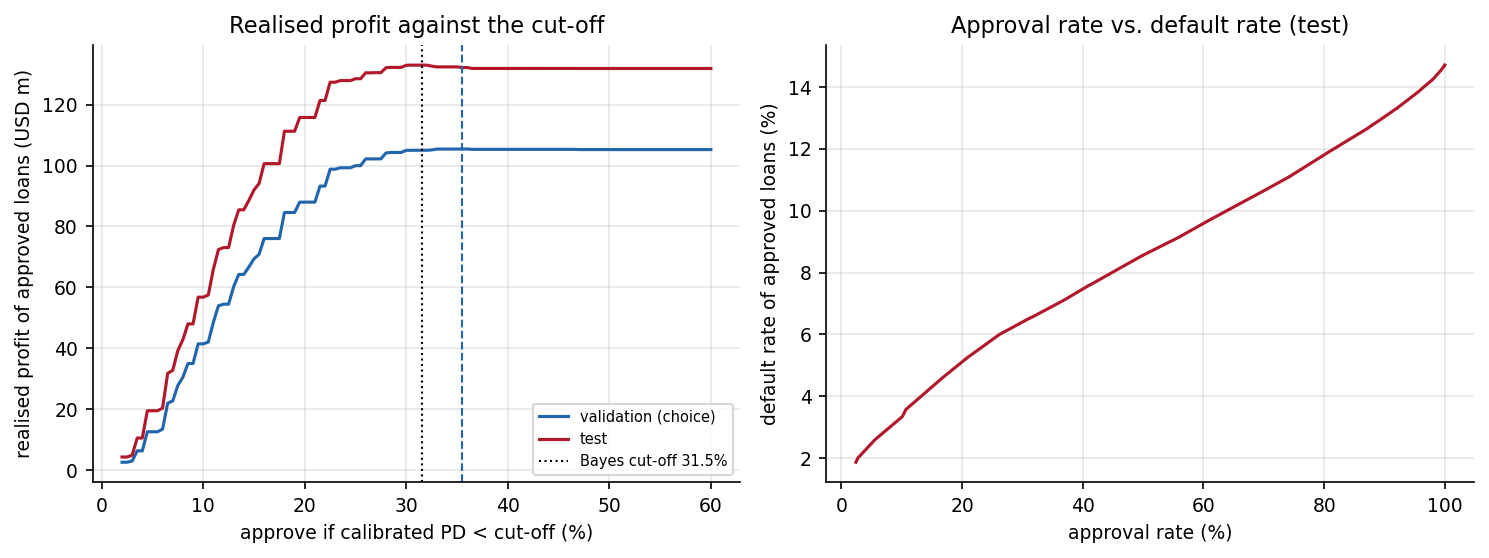
\includegraphics[width=\textwidth]{fig17_threshold.png}
\caption{Left: realised profit of approved loans against the cut-off (validation used for the choice, test for the check). Right: approval rate against the default rate of approved loans.}
\label{fig:threshold}
\end{figure}

\section{Limitations}
\label{sec:limits}
\begin{itemize}
  \item \textbf{Data.} US unsecured peer-to-peer loans of 2007--2015, already screened by Lending Club; the rejected applications are not used (no reject inference). Results do not transfer directly to a European bank's book.
  \item \textbf{Information.} Only the application file is used; Lending Club's grade, which used more bureau data, ranks better (AUC 0.681). No behavioural data (monthly payments, balances) is available, so there is no behavioural score.
  \item \textbf{Default timing and delinquency} are reconstructed from the last payment date. Loans that were late and then cured are invisible, so the stage-2 population and its PD are understated.
  \item \textbf{IFRS~9 simplifications.} One timing curve for every loan; no prepayment in the EAD; undiscounted recoveries; the macro link comes from US bank charge-offs, not from Lending Club, and is weak ($R^2 = 0.08$); scenario weights and shocks are assumptions. The ECL under-predicts the realised loss by 16\%.
  \item \textbf{Fairness.} No protected attribute is in the data; segment checks are a proxy, not a fair-lending test.
  \item \textbf{Tuning budget.} Hyperparameters were searched on 60{,}000 loans with 8 to 20 candidates per model; a larger search would change the third decimal of the AUC, not the conclusions.
  \item \textbf{Cut-off.} Profit ignores funding, operating and capital costs and the time value of money.
\end{itemize}

\section{Conclusion}
On 620{,}779 real loans with a time-based split, gradient boosting and a neural network beat the classic WoE scorecard by a significant but modest 0.023 AUC, and three different flexible models end up statistically tied: the information in the application file, not the algorithm, is the binding constraint. The more useful work for a lender lies around the model: recalibrating on the latest period, which cut the calibration error by a factor of three; explaining each decision with SHAP; monitoring stability; and turning the PD into a term structure, an IFRS~9 allowance and a cut-off. The back-test is the most instructive result: an apparently well-calibrated PD still under-predicted the loss of the following two and a half years by 16\%, because of the simplifications in staging and timing that a production model would have to remove. Natural extensions are a behavioural model on monthly payment data, a survival model for the PD term structure (instead of a single timing curve), a segmented LGD model, and a Lending Club-specific macro model.

\bibliographystyle{plainnat}
\bibliography{references}

\appendix
\section{Reproducibility}
All numbers in this paper are produced by the code in the repository (\texttt{python run\_all.py}): \texttt{scripts/01} downloads the data, \texttt{02}--\texttt{09} prepare the sample, fit the scorecard and the models, calibrate, explain, monitor, compute the ECL and choose the cut-off, and write every result to \texttt{results/*.json}. The random seed is fixed (42). Unit tests (\texttt{pytest}) check the WoE and points arithmetic, the metrics, the calibrators, the PSI, the PD term structure and the annuity schedule, the ECL and the Bayes cut-off on synthetic data.

\end{document}
